\documentclass[11pt]{article}

% ------------------------------------------------------------
% Packages
% ------------------------------------------------------------
\usepackage[margin=1in]{geometry}
\usepackage{amsmath, amssymb}
\usepackage{siunitx}
\usepackage{physics}
\usepackage{graphicx}
\usepackage{tikz}
\usepackage{pgfplots}
\pgfplotsset{compat=1.18}
\usepackage{enumitem}

% ------------------------------------------------------------
% Handy macros
% ------------------------------------------------------------
\newcommand{\T}{T}
\newcommand{\w}{\omega}
\newcommand{\f}{f}
\newcommand{\ymax}{y_{\max}}
\newcommand{\vmax}{v_{\max}}
\newcommand{\amax}{a_{\max}}

\begin{document}

\begin{center}
    {\LARGE \textbf{Simple Harmonic Motion (SHM) --- Algebra-Based Notes}}\\[4pt]
    {\large Mass--Spring Oscillator: Position, Velocity, Acceleration}\\[6pt]
\end{center}

\hrule
\vspace{0.6em}

\section*{1.\ What SHM Looks Like (Big Picture)}
Simple harmonic motion is periodic motion where the restoring force is proportional to the displacement from equilibrium:
\[
F = -ky.
\]
For a mass--spring system, this produces a sinusoidal motion in time.

\subsection*{Key time ideas}
\begin{itemize}[itemsep=2pt]
\item \textbf{Period} $\T$: time for one full cycle.
\item \textbf{Frequency} $\f = \dfrac{1}{\T}$.
\item \textbf{Angular frequency} $\w = 2\pi \f = \dfrac{2\pi}{\T}$.
\end{itemize}

\section*{2.\ Position Function}
If the mass is at its \textbf{maximum height/displacement at $t=0$}, the cleanest choice is a cosine:
\[
y(t)=\ymax \cos(\w t)=\ymax \cos\!\left(\frac{2\pi}{\T}\,t\right).
\]

\subsection*{Why cosine here?}
Because $\cos(0)=1$, so at $t=0$:
\[
y(0)=\ymax.
\]
That matches “starting at maximum.”

\section*{3.\ Velocity Function}
Velocity is the time derivative of position:
\[
v(t)=\dv{y}{t}.
\]
Differentiate $y(t)=\ymax \cos(\w t)$:
\[
v(t)= -\ymax \w \sin(\w t)
     = -\ymax\left(\frac{2\pi}{\T}\right)\sin\!\left(\frac{2\pi}{\T}\,t\right).
\]

\subsection*{Maximum speed}
The sine function ranges from $-1$ to $+1$, so the velocity ranges from $-\ymax\w$ to $+\ymax\w$:
\[
\vmax = \ymax \w = \ymax \left(\frac{2\pi}{\T}\right).
\]
So you can also write:
\[
v(t)=-\vmax \sin\!\left(\frac{2\pi}{\T}\,t\right).
\]

\section*{4.\ Acceleration Function}
Acceleration is the derivative of velocity (or the second derivative of position):
\[
a(t)=\dv{v}{t}=\dv[2]{y}{t}.
\]
Differentiate $v(t)=-\ymax\w\sin(\w t)$:
\[
a(t)= -\ymax\w^2 \cos(\w t)
     = -\ymax\left(\frac{2\pi}{\T}\right)^2
        \cos\!\left(\frac{2\pi}{\T}\,t\right).
\]

\subsection*{Maximum acceleration}
\[
\amax = \ymax \w^2 = \ymax\left(\frac{2\pi}{\T}\right)^2.
\]

\subsection*{Important relationship}
Because $y(t)=\ymax\cos(\w t)$ and $a(t)=-\ymax\w^2\cos(\w t)$:
\[
\boxed{a(t)=-\w^2\,y(t)}
\]
Acceleration always points toward equilibrium (opposite the displacement).

\section*{5.\ Phase Relationships (Who Leads/Lags?)}
\begin{itemize}[itemsep=2pt]
\item $y(t)$ is a cosine wave.
\item $v(t)$ is a negative sine wave: shifted by $\tfrac{\T}{4}$ relative to $y(t)$.
\item $a(t)$ is a negative cosine wave: exactly opposite $y(t)$.
\end{itemize}

\subsection*{Checkpoint times (starting at $y=\ymax$ at $t=0$)}
Let $\theta=\w t=\dfrac{2\pi}{\T}t$.

\begin{center}
\begin{tabular}{c|c|c|c|c}
Time & $\theta$ & $y$ & $v$ & $a$\\ \hline
$0$ & $0$ & $+\ymax$ & $0$ & $-\amax$\\
$\T/4$ & $\pi/2$ & $0$ & $-\vmax$ & $0$\\
$\T/2$ & $\pi$ & $-\ymax$ & $0$ & $+\amax$\\
$3\T/4$ & $3\pi/2$ & $0$ & $+\vmax$ & $0$\\
$\T$ & $2\pi$ & $+\ymax$ & $0$ & $-\amax$
\end{tabular}
\end{center}

\section*{6.\ Quick Sketches (Spring + Graphs)}

\subsection*{Spring--mass diagram (simple)}
\begin{center}
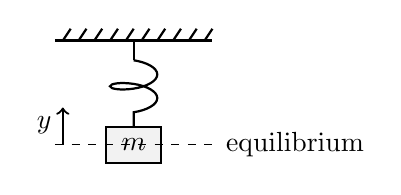
\begin{tikzpicture}[scale=1]
  % ceiling
  \draw[thick] (-1,2) -- (1,2);
  \foreach \x in {-0.9,-0.7,...,0.9}{
    \draw[thick] (\x,2) -- (\x+0.1,2.15);
  }
  % spring
  \draw[thick] (0,2) -- (0,1.75);
  \draw[thick,decorate,decoration={coil,aspect=0.35,segment length=3mm,amplitude=3mm}]
    (0,1.75) -- (0,0.9);
  % mass
  \draw[thick,fill=gray!10] (-0.35,0.45) rectangle (0.35,0.9);
  \node at (0,0.675) {$m$};

  % equilibrium line
  \draw[dashed] (-1,0.675) -- (1,0.675);
  \node[anchor=west] at (1.05,0.675) {equilibrium};

  % displacement arrow
  \draw[->,thick] (-0.9,0.675) -- (-0.9,1.15);
  \node[anchor=east] at (-0.92,0.92) {$y$};
\end{tikzpicture}
\end{center}

\subsection*{Position, velocity, acceleration vs.\ time (one period)}
Below we plot one full period using $\theta=\dfrac{2\pi}{\T}t$ on the horizontal axis.

\begin{center}
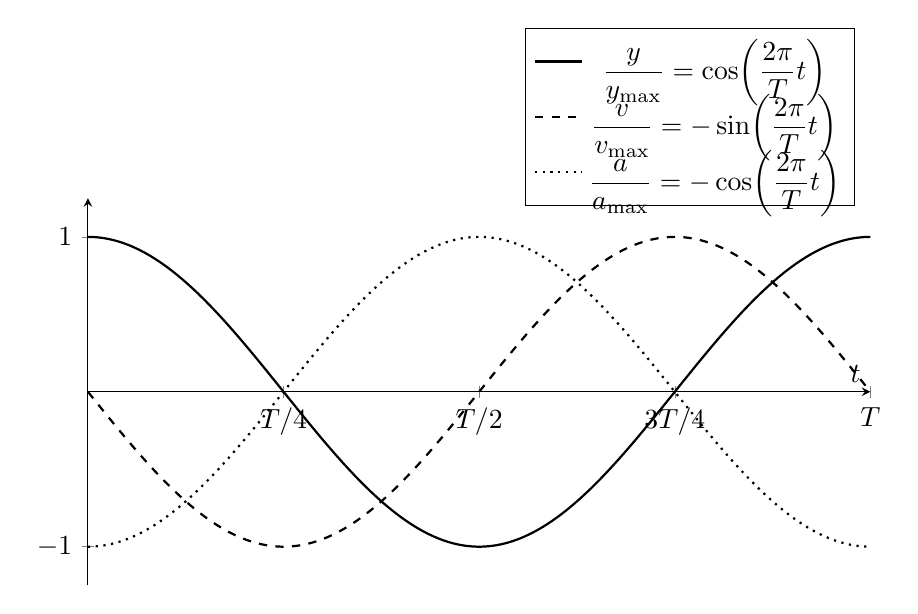
\begin{tikzpicture}
\begin{axis}[
    width=0.95\linewidth,
    height=6.5cm,
    axis lines=middle,
    xlabel={$t$},
    ylabel={},
    xmin=0, xmax=1,
    ymin=-1.25, ymax=1.25,
    xtick={0,0.25,0.5,0.75,1},
    xticklabels={$0$,$\T/4$,$\T/2$,$3\T/4$,$\T$},
    ytick={-1,0,1},
    legend style={at={(0.98,0.98)},anchor=south east},
    samples=200,
    domain=0:1
]
% Use normalized time u=t/T so that one period is u in [0,1]
\addplot[thick] {cos(deg(2*pi*x))};
\addlegendentry{$\displaystyle \frac{y}{\ymax}=\cos\!\left(\frac{2\pi}{\T}t\right)$}

\addplot[thick,dashed] {-sin(deg(2*pi*x))};
\addlegendentry{$\displaystyle \frac{v}{\vmax}=-\sin\!\left(\frac{2\pi}{\T}t\right)$}

\addplot[thick,dotted] {-cos(deg(2*pi*x))};
\addlegendentry{$\displaystyle \frac{a}{\amax}=-\cos\!\left(\frac{2\pi}{\T}t\right)$}
\end{axis}
\end{tikzpicture}
\end{center}

\section*{7.\ Example }
\textbf{Problem.} Write the position equation of a mass attached to a spring with period $\T=\SI{2}{s}$ and maximum height (amplitude) $\ymax=\SI{2}{cm}=\SI{0.02}{m}$. Assume the mass is at maximum height at $t=0$. Draw the position diagram. Also write $v(t)$ and $a(t)$.

\subsection*{Step 1: Find $\w$}
\[
\w=\frac{2\pi}{\T}=\frac{2\pi}{\SI{2}{s}}=\pi\ \text{rad/s}.
\]

\subsection*{Step 2: Position}
Starting at maximum means cosine:
\[
\boxed{y(t)=0.02\cos(\pi t)\ \text{m}}
\]

\subsection*{Step 3: Velocity}
\[
v(t)=\dv{}{t}\bigl(0.02\cos(\pi t)\bigr)=-0.02\pi\sin(\pi t).
\]
\[
\boxed{v(t)=-0.02\pi\,\sin(\pi t)\ \text{m/s}}
\]
Maximum speed:
\[
\vmax=\ymax\w=0.02(\pi)=0.02\pi\ \text{m/s}.
\]

\subsection*{Step 4: Acceleration}
\[
a(t)=\dv{}{t}\bigl(-0.02\pi\sin(\pi t)\bigr)=-0.02\pi^2\cos(\pi t).
\]
\[
\boxed{a(t)=-0.02\pi^2\,\cos(\pi t)\ \text{m/s}^2}
\]
Maximum acceleration:
\[
\amax=\ymax\w^2=0.02(\pi^2)=0.02\pi^2\ \text{m/s}^2.
\]

\subsection*{Position sketch for the example (0 to 2 s)}
\begin{center}
\begin{tikzpicture}
\begin{axis}[
    width=0.9\linewidth,
    height=5.5cm,
    axis lines=middle,
    xlabel={$t\;(\text{s})$},
    ylabel={$y\;(\text{m})$},
    xmin=0, xmax=2,
    ymin=-0.025, ymax=0.025,
    xtick={0,0.5,1,1.5,2},
    ytick={-0.02,0,0.02},
    samples=250,
    domain=0:2
]
\addplot[thick] {0.02*cos(deg(pi*x))};
\end{axis}
\end{tikzpicture}
\end{center}

\section*{8.\ Trig Range Reminder}
Because
\[
-1\le \cos\theta \le 1
\qquad\text{and}\qquad
-1\le \sin\theta \le 1,
\]
the maximum values come directly from the coefficients:
\[
|y|\le \ymax,\quad |v|\le \vmax=\ymax\w,\quad |a|\le \amax=\ymax\w^2.
\]

\vspace{0.5em}
\hrule
\vspace{0.5em}

\begin{center}
\textbf{Core SHM Summary (starting at maximum):}\quad
$\displaystyle y=\ymax\cos(\w t),\;
v=-\ymax\w\sin(\w t),\;
a=-\ymax\w^2\cos(\w t)=-\w^2y$
\end{center}

\end{document}
